\chapter{Associative Arrays} \label{associative}
\section{Introduction}

An associative array is a data structure that lets you manage pairs of data.   Each data pair consists of a key and a value,  where the key is a unique identifier and the value might repeat.  An associative array does not permit the collection of data to have duplicate key values.   For example, if we were storing a collection of data that consisted of student numbers and student names an associative array might be suitable.   Student id numbers are unique within the university so we could guarantee that there would not be any duplicate numbers.  The student number would be the key in this example and the student name would be the value.  It is perfectly permissible for values to repeat.  For example, it is very likely that there would be many students with names like Erin or Lynne.


Student records are a good example of data that is easily stored in an associative array. The student ID (your student number) is the key, and the other data about you (your name, your program, your GPA, etc) forms the value. It is common to have a complex data type (a struct in C) as the value in an associative array.

\section{Implementation}
Associative Arrays can be implemented using a simple array, lists, hash tables and a variety of trees. In this section we look briefly at the array and list implementations. 


\subsection{Array Implementation}

An array implementation of an associative array is useful when the keys for the key/value pairs can be restricted to a finite size and the key of the data pair is  an integer because the keys are used as the indices into the array.         

The picture below shows an array based associative array. The left hand column is just to illustrate the position of the data and would not be stored separately. The 'key' would simply be the index into the array.



\begin{figure}[H]
\centering
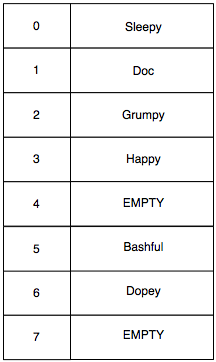
\includegraphics[width=0.3\textwidth]{pictures/image004.png}
\caption{Array Implemented Associative Array}
\label{fig:aa2}
\end{figure}

A sentinel value is used when there is no value for the key (The sentinel values is EMPTY in the example picture).      

\begin{itemize}
\item Advantages:
\begin{itemize}
	\item An array based implementation gives very fast operations because most require only a simple index into the array (O(1)).         
	\item The array based implementation is also simple and easy to understand.
\end{itemize}

\item Disadvantages:
\begin{itemize}
	\item The entire storage space must be created and initialized to EMPTY, meaning that the storage requirements are quite large compared to other implementations, especially if the set of possible keys is large.
\end{itemize}
\end{itemize}

\subsection{Linked List Implementation}


A linked list implementation of an associative array can use  a specialized list node that contains  the key value as an integer as well as pointers to the one to the next item in the list and  the associated value.

Note that there is no \textbf{requirement} to keep a linked list table sorted in any particular order (in the picture below the list is not sorted by the key) but it often improves performance if the list is kept sorted.

\begin{figure}[H]
\centering
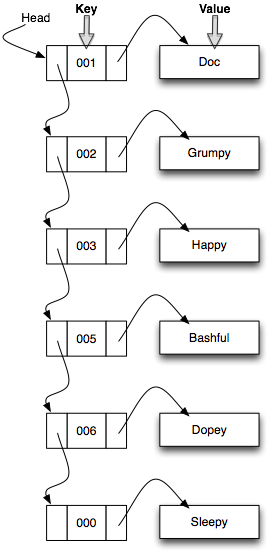
\includegraphics[width=0.3\textwidth]{pictures/image006.png}
\caption{Linked List Implemented Associative Array}
\label{fig:aa3}
\end{figure}

The picture shows a associative array that is a single linked list where the key is stored in the list node along with a pointer to the value. What would be the challenge if you tried to simply use the position of the node in the list as the key? \newline
The struct for a linked version of an associative array might look like this:

\begin{lstlisting}
struct aarray{
    int * key;
    node * next
    void * data
    };
\end{lstlisting}

The reason for adding the key explicitly into the struct rather than leaving it as part of the void*data is that the operations on the array need to compare the key value and would not be able to do that if the key was hidden in the abstracted data.

\begin{itemize}
\item Advantages:
\begin{itemize}
	\item The size of the associative array can grow arbitrarily
	\item The keys do not need to be restricted to a simple integer- for example the key could be a unique alphanumeric
\end{itemize}

\item Disadvantages:
\begin{itemize}
	\item The cost of each operation is dependent on the size of the associative array
\end{itemize}
\end{itemize}

\section{Operations on Associative Arrays}
Operations List (Minimum Set):
\begin{itemize}
	\item create(): AArray
	\item destroy(AArray)
	\item insert (AArray, key, value) 
	\item remove(AArray, key)
	\item lookup(AArray, key):value
	\item update(AArray, key, newValue)
\end{itemize}

\begin{lstlisting}
create():AArray
Purpose: to create an empty, initialized associative array
Preconditions: none
Postconditions: an empty, initialized associative array is created

create():AArray
      1. create the storage ADT
      2. create the key ADT
      3. return(the AArray we just created)
\end{lstlisting}


\begin{lstlisting}
destroy(AArray)
Purpose: to destroy an associative array and free the  memory if required
Preconditions: an initialized associative array
Postconditions: the array  is destroyed along with all references to data. (Important note: the data itself may not be destroyed by this operation and should be removed prior to destroying the AArray).

destroy(AArray)
      1. the appropriate destroy procedure
      2. release any other pointers
\end{lstlisting}

\begin{lstlisting}
insert(AArray, key, value)
Purpose: To add a key/value pair to the associative array
Preconditions: no value exists for the key being added
Postconditions: the size of the AArray has increased by one, the key and value are stored with a reference leading from key to value.

insert(AArray,key,value)
      1. key into key ADT 
      2. connect key and value with reference (pointer)
      3. increase length counter of AArray by one
\end{lstlisting}


\begin{lstlisting}
remove (AArray,key): value
Purpose: to remove a key/value pair from the associative array
Preconditions: the  key/value pair is stored in the AArray
Postconditions: the key/value pair is no longer in the AArray. The length of the AArray has decreased by one.

remove (AArray,key): value
      1. look up key in key ADT
      2. follow reference to value in value ADT
      3. store value in temporary variable
      4. remove value from value ADT
      5. remove key from key ADT
      6. return(temporary variable)
\end{lstlisting}


\begin{lstlisting}
lookup (AArray, key): value
Purpose: to retrieve the value stored for a particular key
Preconditions: the key/value pair is in the AArray
Postconditions: the value is returned. The AArray is unchanged.

lookup (AArray,key): value
      1. look up key in key ADT
      2. follow reference to value in value ADT
      3. store value in temporary variable
      4. return(temporary variable)
\end{lstlisting}


\begin{lstlisting}
update (AArray, key, newValue)
Purpose: the change the value associated with a key that already exists in the associative array
Preconditions: a key/value pair exists for the given key
Postconditions: the new value is associated with the given key


update (AArray, key, newValue)
      1. look up key in key ADT
      2. follow reference to value in value ADT
      3. set value to newValue
\end{lstlisting}


\begin{lstlisting}
exists(key):Boolean
Purpose: to determine if a key is represented in the associative array
Preconditions: an initialized AArray is available
Postconditions: n/a

exists(key):Boolean
      1. look up key in key ADT
      2. if key is found return(true)
      3. else return(false)
\end{lstlisting}


\begin{lstlisting}
isEmpty():Boolean
Purpose: to determine if any key/value pairs are represented in the associative array
Preconditions: an initialized AArray is available
Postconditions: n/a

isEmpty():Boolean
      1. if the key ADT is empty; return(true)
      2. else return (false)
\end{lstlisting}


\begin{lstlisting}
isFull():Boolean
Purpose: to determine if the AArray is full
Preconditions: an initialized AArray is available
Postconditions: n/a

isFull():Boolean
      1. if the key ADT is empty; return(true)
      2. else return (false)
\end{lstlisting}


\section{Applications}
Associative arrays are useful in any situation where you need to maintain a connection between two pieces of data, but where the data might be changed frequently during the running of the program. As an abstract example, AArays are less appropriate for connections between a person and their phone number- which typically stays the same, and more appropriate for representing the connections between a parking lot ticket number on a vehicle and a parking spot.    

Associative arrays are really only useful if the  key portion of the key-data pair maps nicely to the positions in an array.   This is most likely to occur in situations where data is generated sequentially,  such as ticket numbers for a coat check,  or order numbers for an online store.

\subsection{Lending Library}

Scenario: Suppose you wanted to implement a lending library for your collection of computer games so that each game could only be lent out to one person at a time (no copies allowed). The core data structure used by this application could be an associative array.


Requirements: 
\begin{itemize}
	\item Each computer game is assigned a unique ID number (0-N)
	\item Borrowers can have more than one game checked out at a time
	\item A game can only be checked out by a single borrower at any one time
\end{itemize}

\subsubsection{Context}

The application would obviously need some user interface constructs to enable data entry and some file storage utilities to permit persistent storage. For the purposes of this example, we will assume those details have been worked out already.


Programming Constructs we would need to write this program
\begin{itemize}
	\item A way of creating borrowers
	\item A way of identifying borrowers 
\begin{itemize}
	\item The set of borrowers will also need to be in an ADT. If you give each borrower an ID, then an AArray might be a good choice for this as well.
\end{itemize}
	\item A way of creating and populating the list of games that can be borrowed
	\item The AArray representation for the set of borrowed games
\end{itemize}


\subsubsection{Worked example}

Lending Library pseudocode
\begin{itemize}
	\item Create and populate borrowers data structure
	\item Create and populate the games data structure
	\item Initialize the AArray  of borrowed games to empty
	\item If a game is borrowed add the game/borrower pair to the AArray representing the borrowed games
	\item if a game is returned remove the game/borrower pair from the AArray representing the borrowed games
\end{itemize}


\section{Extending Activities}
\begin{itemize}

\item {
If you were implementing a student record system for a small music  school with fewer than 200 students, and were using associative arrays as the data structure, how would you implement your associative array? Would you make a different choice if your student record system was for a university?

}

\item {
Write a 'todo list' of the things you would need to do (including research and learning) in order to implement the borrowers library example.Try to make the list very specific. Use the todo list to estimate the amount of time it would take you to implement and test the application (round up to the nearest hour).
subsubsection

}

\end{itemize}
\chapter{Hash Tables} \label{hash}
\section{Introduction}
 
A Hash Table is an array (aka Table) that uses a hash function to map keys to a specific location in the array.   The position of the entry in the table is determined by the value of the key.  
 
 A hash table (also knowns as a Hash Map)  is a more flexible version of an associative array that does not require that the key of the the key-data pair be something that easily maps to a position in a table.   Instead, the hash table calculates the table position by algorithmically manipulating (hashing) the key to determine the correct position in the table.   A hash table is useful in situations where the data key-value pairs might not have key values that are nicely distributed to allow them to be mapped to table positions between 0 and the end of the table.
 
 
The \textbf{Hash Function} a function that, when given a key as a parameter returns  an integer within a  fixed range.   The hash function ALWAYS returns the same value for a given input, but may return the same value for more than one input.   For example,  a hash function could take in the province and plate number from a car licence plate (something like ONBWCC123) and manipulate the digits and letters to produce an integer that maps to a position on the table.  If the hash table were of size 357, the integer would be between 0 and 356.  

\begin{figure}[H]
\centering
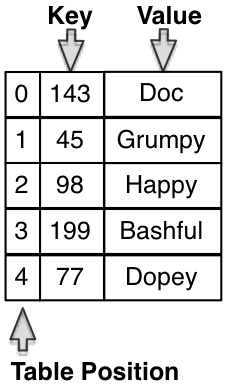
\includegraphics[width=0.3\textwidth]{pictures/Hash_Tables_0.png}
\caption{Hash Table}
\label{fig:hashTable}
\end{figure}

Image \ref{fig:hashTable} shows a 3x5 table.  The first column is labeled as Table Position, the second shows the key, the third shows the value.  There are five sets of data in the table.  

The hash table shown is a simplified table that has the data stored directly in the table.  A finished implementation of a hash table ADT would store void * data in the same way that a linked list does.   A hash table is nearly always implemented using an array, since the primary purpose of using a hash table to facilitate speedy lookups for data.

\paragraph{Real World Example:}
 
Spelling checkers are an application that can employ a hash table.   Because the dictionary of properly spelled words can be quite large,   a search through that dictionary for each word in the document being checked is the most time consuming part of the operation.   The dictionary can be read once into a hash table, where each word in the dictionary is put through a hash function and stored in the table at the appropriate position.  In this example the word is both the key AND the data.
After the table is loaded each word of the document to be spell checked is hashed

\section{Hash Table Operations}
The minimum set of operations for a hash table are exactly the same as the operations for an associative array.
     
The only change is the process for inserting and finding data because the hash table must use the hash function to determine where the new data goes and where the data can be found.
   
The implementation of the operations changes depending on the collision resolution strategy chosen.

Operations List (Minimum Set):  
This is exactly the same operations list is for an associative array.   The algorithms for the operations are also the same and are not repeated here.
\begin{itemize}
\item create(): HTable
\item destroy(HTable)
\item insert (HTable, key, value)
\item remove(HTable, key)
\item lookup(HTable, key):value
\item update(HTable, key, newValue)
\end{itemize}


\section{Hash Table Characteristics}

Hash tables are relatively simple to implement and provide operations that are ideal for tasks that involve frequent look ups of the elements.  Hash tables have several characteristics that  distinguish them from other data structures.


\begin{itemize}
\item Hash tables can provide an improvement over the search time for binary trees ( binary tree search time is O(log 2 n).     The cost of search in a hash table is the time to execute the hash function + any time to resolve collisions which is usually O(1).
\item Hash tables are efficient for large sets of data, but sometimes the hash function is computationally expensive which makes other data structures more effective for small sets of data.
\item The most often used operations on a hash table are the operations for finding and inserting.   These operations are dependent on the hash function.   The selection of hash function is key to the efficient operation of the hash table.
\item The set of keys for the data is called the key space.   The key space is often larger than the size of the table in memory (the address space), which means that often two elements must hash to the same location.  When this happens the collision resolution strategy is used to ensure that both elements are stored and can be retrieved.

\item The hash function maps the key space into the address space.   More specifically the hash function takes a key and uses it to produce an address that is in the defined address space of the allocated table.   The same address must be produced every time given the same key.
\item Because the key space is typically larger than the address space, more than one key will be mapped to the same address.   This is called a collision and must be handled through collision resolution. The selection of collision resolution method is an important part of hash table design.
\end{itemize}


\section{Hash Functions}

The hash function must map the keys in the data to a position in the table.   A hash function needs to know the size of the table (usually sent in as a parameter) in order to determine the appropriate position.
     
The characteristics of a good hash function are:
\begin{itemize}
\item speed: the function cannot be slow to run
\item space: the hash function should not take a lot of storage space
\item generation of positions: the function should spread the keys out evenly across the whole hash table (no clustering in one part of the table)
\end{itemize}

All hash functions take in a key of a particular type as a parameter and return a value between 0 and the size of the table.   Some hash functions are written with a hard coded table size,  some take the table size as a parameter.  Some hash functions work on numeric keys,  some work on alphanumerics.   There are many different possible hash functions.  The subsections below detail some possible approaches to writing hash functions.

\subsection{Before Hashing: Preconditioning}

     Keys in the key space frequently contain alphanumeric characters, but hash functions are often more effective on keys that can be manipulated numerically. One common approach to hashing is to convert alphanumeric keys to a numeric value through a process called preconditioning. Preconditioning can be as simple as replacing each letter with the ascii code for the  letter, or it can do more complex manipulations such as normalizing the length of the keys in addition to converting them. 
   
\subsection{ Hashing by Truncation}

    The \textbf{truncation} method of hashing simply uses a portion of the key as the 
       address space and ignores the rest of the key.  This method is also known as \textbf{Digit Analysis}
       

     The truncation method only works for keys that have consistent characteristics.  For example, suppose you had a set of 8 digit keys such as 46 234 789 and your hash table size was 1000 (hash values between 0 and 999).
     
     One approach to truncation for hashing this number could be to simply select the 1 $^st$ , 3 $^rd$ and 5 $^th$ digits of the key (424 in this case). Another approach to truncation for hashing this type of key could be to select the first, third and last digits and then reverse the order (924 in this case).
     
The approach to truncation must be consistently applied to every key and must always give the same results, but otherwise any sort of digit manipulation that results in a suitably sized address space can be considered as an approach to truncation.

The truncation method has the advantage that it is very fast, but it often results in many collisions because the hashed values often don’t distribute well within the entire table.

\subsection{Hashing by Folding}

The \textbf{folding method} of hashing involves separating the key into parts that are the same length as the address space and performing some kind of math on those parts.  Often one part is composed of the ‘leftovers’ and is a different length.  A common method of folding is to add the parts together once the parts are identified, ignoring the final carry.   The result is used as the table address for the original key.


For example, suppose that the key value of 456 987 321 must be hashed into a table of size 1000 (hash values between 0 and 999). The original key is partitioned into three segments, each three digits long and those segments are added together. 456 + 987 + 321 = 1764. The 1 thousand is ignored and the hash key becomes 764.

The folding method is a fast hashing algorithm and results in more evenly distributed addresses than truncation.  Even though it is better than truncation, it can still result in poorly distributed addresses.

\subsection{Hashing by Division}

Integer division can be used to consistently reduce a large integer to a small one.  Recall the modulo operator, which is used to find the remainder value after integer division.   15 modulo 4 (15\%4) yields the value 3.    The only possible values from an expression that is modulo 4 is 0, 1, 2 or 3.    If we use larger numbers,  say 10000 modulo 999,  the remainder value will have to be  a number between 0 and 998.  We can use this characteristic of  modulo to calculate a hash value of a large number.

The division method hash function calculates the hash value of a key, H(k) by finding the remainder that results from dividing k by some positive integer (modulo). More formally \textbf{H(k) = ABS(k)\%m} where m is a large positive integer, \% is the modulo operator and ABS is the absolute value.

 The division method of hashing will return addresses that are between zero and one less than the divisor (m), so it is important that m is also the size of the table, otherwise this method will result in invalid addresses.


 This method will map keys that are close in value to different addresses, but will map keys that are multiples of each other to the same address, so its effectiveness depends on the characteristics of the original key space. Consider the hash values calculated below, for an m value of 11.
   


\begin{tabular}{lllll}
\hline
Key & Hash  \\ \hline
12  & 1     \\
13  & 2     \\
14  & 3     \\ \hline
56  & 1     \\
57  & 2     \\
58  & 3     \\
239 & 8    
\end{tabular}

The division method can result in very good distribution of address locations depending on the value chosen for m.  The table size (m) should not be set to an even number, or a power of 2 or 10.   Prime numbers, and odd numbers  whose factors are all over 20 are good choices for the table size (m).
   

\section{Collision Resolution for Hashing}

When two keys hash to the same table position we say that a \textbf{collision} has occurred.  Even if the keys for the data are unique, it is likely that sometimes the hash function will calculate the same table position for two keys.   When  this happens, the hash table must find a different location to store the second set of data, since two pieces of data cannot be stored in the same memory location.   The process of locating the alternate storage location is called \textbf{collision resolution}.
   
Two common approaches to collision resolution are \textbf{open addressing} and \textbf{separate chaining}.  Open addressing solutions use an algorithm to search in a repeatable fashion for an alternate location.   Separate chaining solutions create additional table space by using a linked data structure.

\subsection{Open Addressing}

     When a collision occurs in an open addressing hashing system, the collision is resolved by trying alternative cells until an empty cell in the hash table is found. In effect some number is added to the calculated cell position to arrive at a new cell to try, and the formula is set to wrap-around to the beginning of the table when the end is reached.
   
     The number of filled cells in the hash table is used to calculate the \textit{load factor} of the table (number filled/size of table). Open addressing is a collision resolution technique that works best with a table that has a load factor of .5 or less.
   
     The offset is calculated by a collision resolution algorithm. A collision resolution algorithm must ensure that it always finds an empty cell if one is available. We will examine three open-addressing collision resolution algorithms that are used : linear probing, random probing, and double hashing.   There are many more possible approaches and several variations on the three we will examine, but these three serve to illustrate the concepts behind open addressing to resolve collisions.
   
Suppose that the items in the table are names.
\begin{itemize}
\item Sleepy is hashed to position 0
\item Doc and Grumpy are hashed to position 3
\item Sneezy is hashed to position 4
\item Happy is hashed to position 5
\item Bashful and Dopey are hashed to position 7
\end{itemize}



The table state, after each addition is shown in the diagram below.


\begin{figure}[H]
\centering
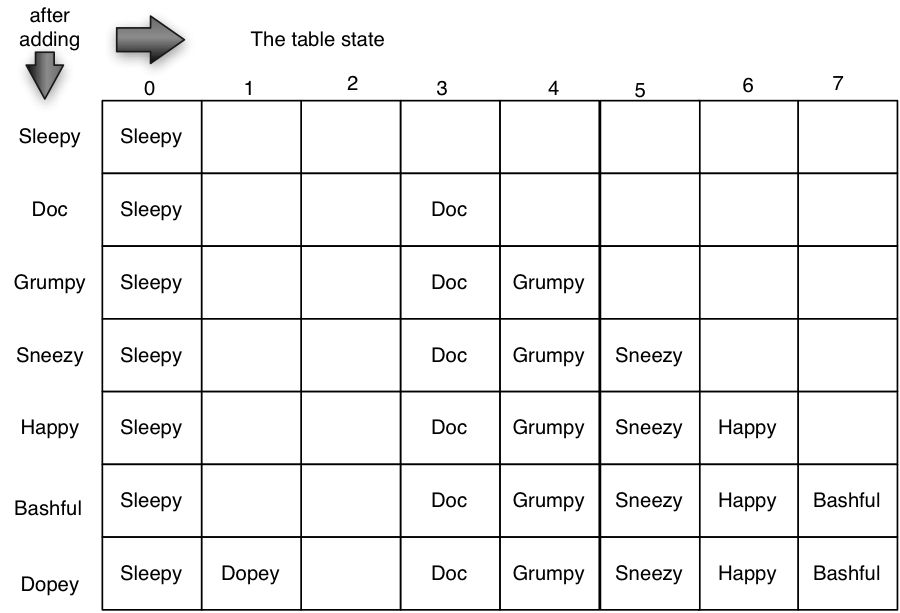
\includegraphics[width=0.5\textwidth]{pictures/Linear_Probing_0.png}
\caption{Linear Probing}
\label{fig:linearProb}
\end{figure}


 While linear probing always finds a cell if one is available, it tends to cluster the data (as you can see in the diagram). This type of clustering is called \textbf{primary clustering}. Also,  as the table gets full, the number of probes required increases which slows down insertions and searching.
   
\subsubsection{Random Probing}


 One way to avoid primary clustering is to change the probing mechanism so that it does not return consecutive positions. The probing strategy cannot truly be random because must still generate every position in the table exactly once for any given collision, and it  must generate exactly the same sequence again given the same collision.  However, it does not  need to generate new table positions  in the order that they appear in the table.
   
One example of such a strategy adds some positive number  to the  location of the collision, and then finds the modulo value with respect to the table size.

\begin{lstlisting}
{ newLocation = (mostRecentLocation + constant) mod tableSize}
\end{lstlisting}


This strategy works well when the constant and the tableSize share no common divisor other than 1. Random probing suffers from \textbf{secondary clustering}.   Secondary clustering occurs when the same exact sequence of  positions is generated   when two keys are mapped to the same position more than once during a search for position. 
   


\subsubsection{Double Hashing or Rehashing}

Double hashing is an effective collision resolution strategy that avoids clustering. When there is a collision of hashed values for keys, the colliding key is hashed again using a different hash function.   The result of the second hash function is not used as a position, but is used as  the constant value in the equation for random probing.
   
\begin{lstlisting}
newLocation = (mostRecentLocation + valueFromSecondHashFunction) mod tableSize
\end{lstlisting}



\subsubsection{Linear Probing}

     Linear probing is a strategy that  places the collided data in the next available cell.  When the end of the table is reached, the search wraps around to the beginning of the table.
     




Double hashing usually eliminates clustering in the hash table because the sequence of values generate for any two colliding keys will not be the same.





\subsection{Separate Chaining}


 Separate chaining is another approach for handling hashing collisions. Rather than try to find an alternate table position, the separate chaining approach stores  the colliding records for a single table  position in a linked list.  Instead of storing data directly in the hash table, the linked list is stored in the hash table at the hashed position.   The separate chaining method requires memory storage space for the hash table as well as for the linked lists, so it is more memory intensive than an open addressing approach to collision resolution.  
   


\begin{figure}[H]
\centering
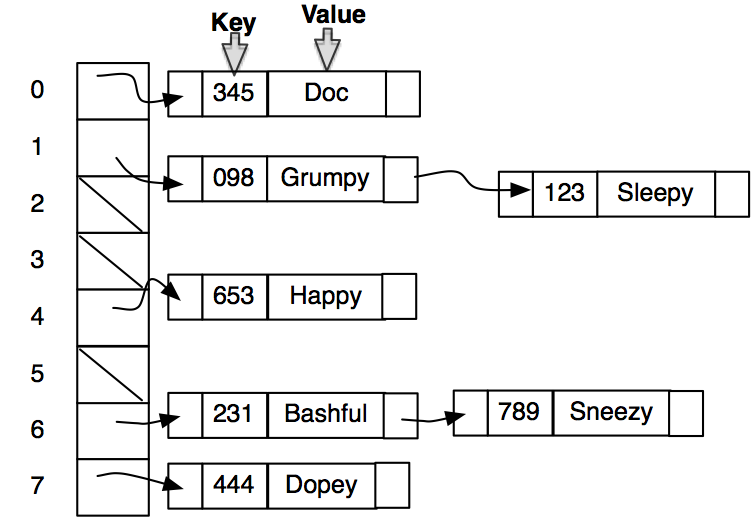
\includegraphics[width=0.5\textwidth]{pictures/Separate_Chaining_0.png}
\caption{Separate Chaining}
\label{fig:sepChain}
\end{figure}




     Separate chaining is often implemented so that none of the data items are stored in the actual hash table.
     Instead the hash table simply houses pointers to the linked lists of data that hash to that location.
     

     Algorithms for separate chaining are easy to construct, as the first step is a simple lookup in an array and the rest of the data structure can be manipulated through linked list operations. If the hash function is good, there will be few collisions and the linked lists will be short.
   
Even though this technique requires more storage space than an open addressing approach, the simplicity and its performance make it a popular choice in hash table design.


\section{Additional Resources}
An excellent hashing tutorial with several animations can be found here:      

       http://research.cs.vt.edu/AVresearch/hashing/

       This tutorial reviews most of what we have learned in this lesson, and        expands the topics somewhat. The animations are excellent and worth exploring.   
       
 \section{Extending Activities}
\begin{itemize}


\item {
Using the division method, calculate hash values for the following set 
       of keys. Calculate once using a table size of 11. Calculate a second 
       time using a table size of 12. do you notice anything about the 
       distributions of the calculated values?



Keys: 54 77 82 13 991 308 68 45 1001 73

}
x
\item {
     The expected search time for Linear probing can be calculated by the following formula:
   
\textbf{ O(1 + 1/(1-loadFactor)) } for a successful search and \textbf{O(1+1/(1-loadFactor)\^2)}  for an unsuccessful search.
     
     Create a chart showing the expected search times (successful and unsuccessful) for the following load factors: .10, .20., .30, .40, .50, .60, .70, .80, .85, .90, .95.
     
     What do these numbers tell you?

}
\item {

     Suppose you have two hash functions H1 and H2  where H1(87) = 10, H2(87) = 3  and  H1(42)=10, H2(42)=7.
     Further suppose that the key 87 is inserted into the table first and then the key of 42.  Show the sequence of table positions tried when using random probing with a constant of 37 and a table size of 11.
     
}
\item {

The expected time for a search using Double hashing can be calculated as shown below:

successful search:  (1/loadfactor)(1+ ln(1/(1-loadfactor))) 

unsuccessful search:  1/(1-loadfactor) 
     
     Calculate a chart of the predicted search times (successful and unsuccessful) for the following load factors: .10, .20., .30, .40, .50, .60, .70, .80, .85, .90, .95.
     
     What do these numbers tell you?
}

\item {

The loadFactor of a hash table using separate chaining to resolve collisions is calculated as the \textbf{number of keys/ the number of chains}
The expected length of search ,  successful or unsuccessful, of Separate Chaining is O(1+loadFactor).  

     
     Calculate 
       a chart of the predicted search times for the following load 
       factors: .10, .20., .30, .40, .50, .60, .70, .80, .85, .90, .95.
     
     What 
       do these numbers tell you?
}

\item {

What factors would you consider when selecting a collision resolution approach for a hash table?

}


\end{itemize}



